\documentclass[11pt]{article}
\usepackage[margin=1in]{geometry}
\usepackage[T1]{fontenc}
\usepackage[utf8]{inputenc}
\usepackage{booktabs}
\usepackage{enumitem}
\usepackage{hyperref}
\usepackage{longtable}
\usepackage{tabularx}
\usepackage{xcolor}
\usepackage{tikz}
\usetikzlibrary{arrows.meta,positioning}
\hypersetup{colorlinks=true,linkcolor=blue,urlcolor=blue,citecolor=blue}
\setlength{\parskip}{0.65em}
\setlength{\parindent}{0pt}

\title{EMA-AI Architecture Report: Local MVP Architecture and Azure Pilot Path for Engineering Readiness Intelligence}
\author{EMA-AI Project Team}
\date{\today}

\begin{document}
\maketitle
\tableofcontents
\newpage

\section{Abstract}
EMA-AI is a local MVP that combines a Revit add-in, landing-root file processing, a FastAPI backend, PostgreSQL persistence, and a React/Vite dashboard to support engineering deliverable readiness. The architecture emphasizes deterministic readiness, explicit operator control, and evidence-candidate labeling rather than official compliance claims.

\section{Architecture Overview}
The system is intentionally layered. Revit prepares exports and landing folders, FastAPI discovers and ingests the landing root, PostgreSQL stores official records, and the dashboard displays portfolio state, processing operations, documents, requirements, issues, and readiness. AI and semantic retrieval are optional advisory layers only.

\begin{center}
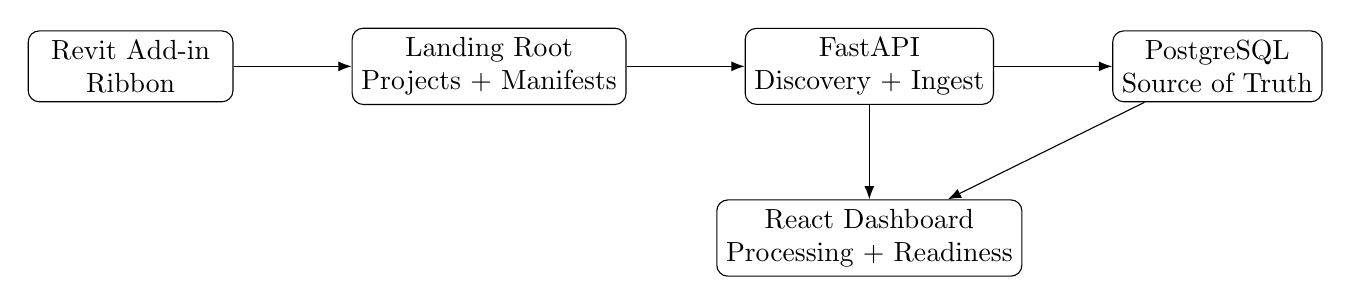
\begin{tikzpicture}[
  node distance=1.2cm and 1.5cm,
  box/.style={draw, rounded corners, align=center, minimum width=2.6cm, minimum height=0.9cm}
]
\node[box] (revit) {Revit Add-in\\Ribbon};
\node[box, right=of revit] (landing) {Landing Root\\Projects + Manifests};
\node[box, right=of landing] (api) {FastAPI\\Discovery + Ingest};
\node[box, right=of api] (db) {PostgreSQL\\Source of Truth};
\node[box, below=of api] (ui) {React Dashboard\\Processing + Readiness};
\draw[-{Latex}] (revit) -- (landing);
\draw[-{Latex}] (landing) -- (api);
\draw[-{Latex}] (api) -- (db);
\draw[-{Latex}] (db) -- (ui);
\draw[-{Latex}] (api) -- (ui);
\end{tikzpicture}
\end{center}

\section{Component Inventory}
\begin{longtable}{@{}llp{7.6cm}@{}}
\toprule
Layer & Component & Responsibility \\
\midrule
\endhead
Edge & EMAExtractor & Local Revit export and landing guidance \\
Backend & FastAPI app & Landing discovery, ingest, readiness, logs, and documents \\
Data & PostgreSQL & Official records, snapshots, issue tracking, readiness data \\
Frontend & React/Vite dashboard & Operator control and executive visibility \\
Docs & Markdown + LaTeX & Procedures, contracts, memory, and publications \\
\bottomrule
\end{longtable}

\section{Runtime Topology}
The local runtime uses Docker for the backend and database, and a Vite development server for the frontend. The same code paths support local demonstration and operator validation.

\section{Local Development Topology}
The developer workflow keeps landing files outside the repository history, uses local configuration for demo state, and treats generated outputs as disposable. This makes the repository usable for review without mixing source control with live project artifacts.

\section{Backend API Architecture}
The backend exposes project, client, landing, document, readiness, issue, dev, and debug endpoints. Landing batch APIs now support full-root discovery, manifest rebuilds, ingest-all, and explicit project/client binding, while preserving dry-run defaults and partial-failure safety.

\section{PostgreSQL Data Model}
The persistence layer centers on project, client, model, export, issue, landing document, requirement, snapshot, and action records. The database is the source of truth for readiness and the audit trail for operator operations.

\section{Landing Root and File Classification}
Files are classified by folder and extension, with sidecars kept separate from documents. Revit exports, drawings, owner requirements, and specifications each have their own semantic treatment. Unknown files do not crash the pipeline; they are reported and skipped.

\section{Revit Add-in Integration Boundary}
The add-in is a preparation layer, not the readiness engine. It exports, opens folders, and steers the operator to the correct workflow. It must not parse PDFs, and it must not claim readiness or official compliance.

\section{Frontend Dashboard Architecture}
The dashboard is route-based and stateful. Its main job is to present readable operator surfaces, protect against render crashes, and keep local demo truth visible: candidate evidence, local demo state, and non-production boundaries.

\section{Processing / Sync Control Plane}
Processing / Sync orchestrates scans, manifest rebuilds, dry-run ingest, real ingest, snapshot creation, and diagnostic refreshes. It is designed for human control and must not be mistaken for autonomous ingestion.

\section{Readiness Engine}
Readiness is deterministic. Requirement coverage, QA/QC health, and sync freshness are combined into a transparent score. Missing requirements remain visible, and not-applicable items are excluded from the denominator.

\section{Observability and Debugging}
Operation logs, debug payloads, environment diagnostics, and endpoint checks are first-class parts of the architecture. They exist so operators can understand what changed and why.

\section{Security Model}
Security is conservative: local demo users are not production auth, sensitive content is not echoed into docs, and path traversal is rejected. Evidence candidate status is preserved until a deterministic workflow promotes records.

\section{Data Governance}
EMA-AI keeps the distinction between raw source files, indexed metadata, evidence candidates, and official records. That distinction matters for reviewers and for future Azure migration planning.

\section{Azure Pilot Architecture}
\begin{tabularx}{\textwidth}{@{}lX@{}}
\toprule
Service & Recommendation \\
\midrule
Frontend & Azure Static Web Apps or App Service \\
Backend & Azure Container Apps or App Service \\
Database & Azure PostgreSQL Flexible Server \\
Files & Azure Storage or Data Lake Gen2 \\
Secrets & Azure Key Vault \\
Observability & Application Insights + Log Analytics \\
Identity & Managed Identity + RBAC \\
\bottomrule
\end{tabularx}

\section{Azure Resource Recommendation}
The Azure pilot should be introduced only after local smoke is stable. It should preserve the deterministic readiness engine and should not claim production security or official compliance.

\section{Deployment Options}
Two deployment styles are practical: a container-first deployment with a single backend service and database, or a slightly more separated frontend/backend arrangement. The MVP should prefer the simplest topology that preserves traceability.

\section{Scalability Considerations}
The main scalability pressure points are document indexing, PDF metadata parsing, and export volume. These can be incrementally improved without changing the local MVP semantics.

\section{Failure Modes}
Known failure modes include missing client binding, path mismatches between host and container, parser unavailability, and incomplete landing folders. The system should degrade to clear empty or warning states rather than a blank page.

\section{Validation and Test Strategy}
The repository currently records 246 C\# add-in tests passing and 127 backend tests passing without the database stack, with 47 additional backend tests still requiring Docker/PostgreSQL. The remaining important validations are manual browser route smoke and Revit runtime smoke.

\section{Open Risks}
\begin{itemize}[leftmargin=*]
\item Manual browser smoke remains pending unless executed.
\item Revit runtime remains pending unless executed in the host application.
\item Azure deployment is a recommendation path only.
\item APS production viewer support is future work.
\end{itemize}

\section{Implementation Roadmap}
The near-term roadmap is straightforward: stabilize the route UX, complete landing-root operator workflows, harden PDF parsing, and document the Azure pilot path without promising production status.

\section{Conclusion}
EMA-AI has a coherent local architecture for deliverable readiness. The most valuable property of the architecture is not its visual polish, but its honesty about evidence, readiness, and operational limits.

\nocite{*}
\bibliographystyle{plain}
\bibliography{references}
\end{document}
